\begin{figure}%
	\centering%
	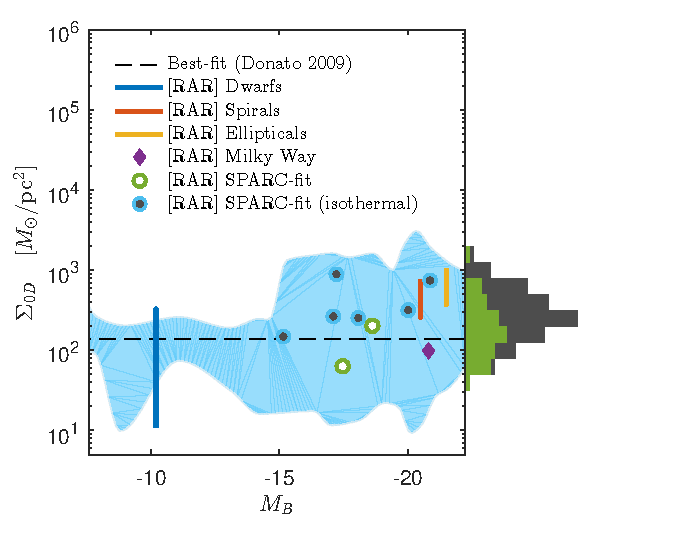
\includegraphics[width=\hsize]{\ROOTPATH/fig.pdf}
	\caption{Prediction of the surface density for disk galaxies of valid SPARC samples. The absolute magnitude was taken from the Carnegie-Irvine Galaxy Survey, providing eight overlapping galaxies. The blue region indicates the delimited area by the $3\sigma$ error bars of all the data points used in \citet{2009MNRAS.397.1169D}. The shown candidates include isothermal (blue outlined points) and non-isothermal (green circles) solutions, which are very well in agreement with the DM surface density observations. For comparison, the results are amended by RAR predictions for typical dwarfs, spirals and ellipticals \citep{RAR-II}. Although absolute magnitude information is incomplete, the predicted DM surface densities of the entire valid galaxy sample is within the range if the $3\sigma$ area as well. These full results are presented in a histogram (grey bars) with comparison to a subsample, including non-isothermal solutions (green bars). The majority of the latter sample is closer the the observationally inferred mean value of about $140 M_\odot$~pc$^{-2}$.}%
	\label{fig:SPARC:Donato}%
\end{figure}